\section{\textsc{French Dressing}}

\subsection*{Zutaten für 100ml:}

\begin{tabular}{p{7.5cm} p{7.5cm}}
	& \\
	40ml Essig & französischer Senf \\
	60ml Öl & Knoblauch \\
	Salz \& Pfeffer &
\end{tabular}

\subsection*{Serviervorschlag:}

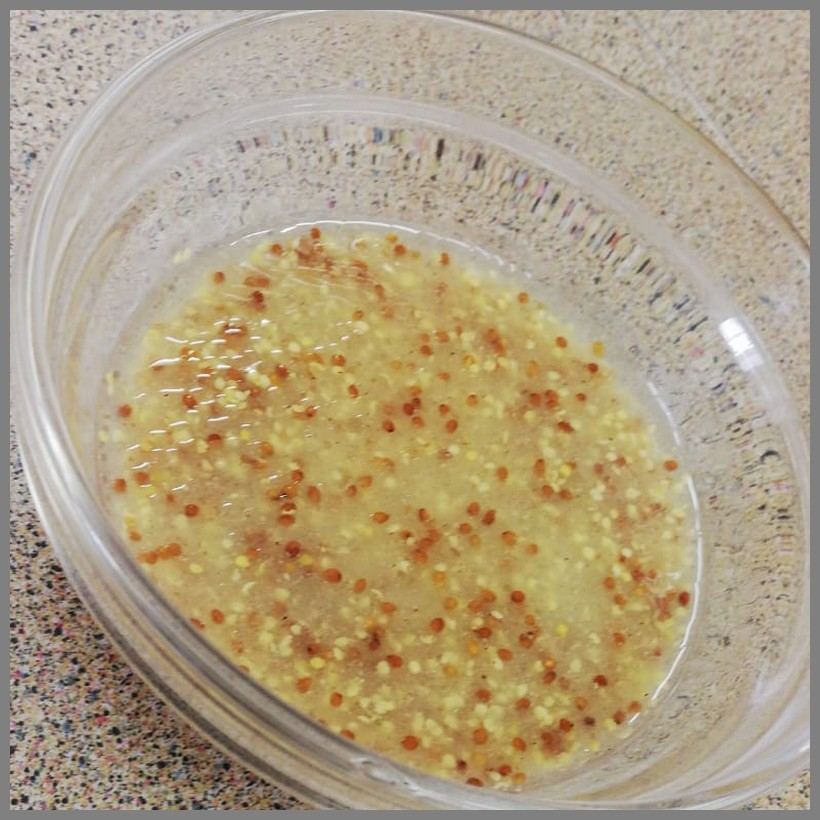
\includegraphics[width=\textwidth]{img/d_french.jpeg} \cite{dfrench}

\subsection*{So geht's:}

\begin{tabular}{p{15cm}}
	\\
	Salatschüssel mit der Schnittfläche einer halbierten Knoblauchzehe einreiben.\\
	Salz, Essig \& Senf darin verrühren.\\
	Langsam das Öl dazugeben und verrühren.\\
	Mit wenig Pfeffer abschmecken.\\
	\\
	Geeignet zu Blattsalat und Gemüsesalat.
\end{tabular}
